\documentclass[aspectratio=169]{beamer}

% --- PAQUETS ---
\usepackage[utf8]{inputenc}
\usepackage[T1]{fontenc}
\usepackage[french]{babel}
\usepackage{graphicx}
\usepackage{graphbox}
\usepackage{booktabs}
\usepackage{tikz}
\usepackage{caption}
\usepackage{amssymb} % Pour \mathbb{E} si besoin

% --- THÈME ---
\usetheme{Madrid} 
\usecolortheme{whale} 

% --- CONFIGURATION DES IMAGES ---
\graphicspath{{images/}} 

% --- INFORMATIONS ---
\title[Robotique \& IA - Soutenance Finale]{Robotique et IA en environnements complexes}
\subtitle{Exploration et détection de fissures en galerie souterraine}
\author[Guichard, Lefebvre, Dame, Paris]{Vincent GUICHARD, Adrien LEFEBVRE\\Lucas DAME, Paul-Antoine PARIS}
\institute[Mines Nancy]{École des Mines de Nancy \\ Partenaire : ANDRA}
\date{Soutenance Finale - Juin 2026}

% --- LOGOS PAGE DE TITRE ---
\titlegraphic{
    \vspace{-0.5cm}
    
\includegraphics[align=c, height=1.2cm]{logo_andra.png}%
    \hspace{0.5cm}
    
\includegraphics[align=c, height=2.2cm]{logo_mines_nancy.png}%
}

\begin{document}

% --- TITRE ---
\begin{frame}
    \titlepage
\end{frame}

% --- SOMMAIRE ---
\begin{frame}{Sommaire}
    \tableofcontents
\end{frame}

% --- SECTION 1 : RAPPEL DU CONTEXTE ---
\section{Objectifs et Architecture}

\begin{frame}{Problématique : Inspection du projet Cigéo}
    \begin{columns}
        \column{0.6\textwidth}
        \textbf{Le besoin de l'ANDRA :}
        \begin{itemize}
            \item Surveiller 270 km de galeries à 500m de profondeur.
            \item Détecter les fissures liées au cisaillement géologique.
            \item Remplacer une inspection manuelle chronophage.
        \end{itemize}
        \vspace{0.3cm}
        \begin{block}{Objectif Final}
            Un système robotisé capable de naviguer de manière autonome et de cartographier les fissures via IA.
        \end{block}
        
        \column{0.4\textwidth}
        \begin{figure}
            \centering
            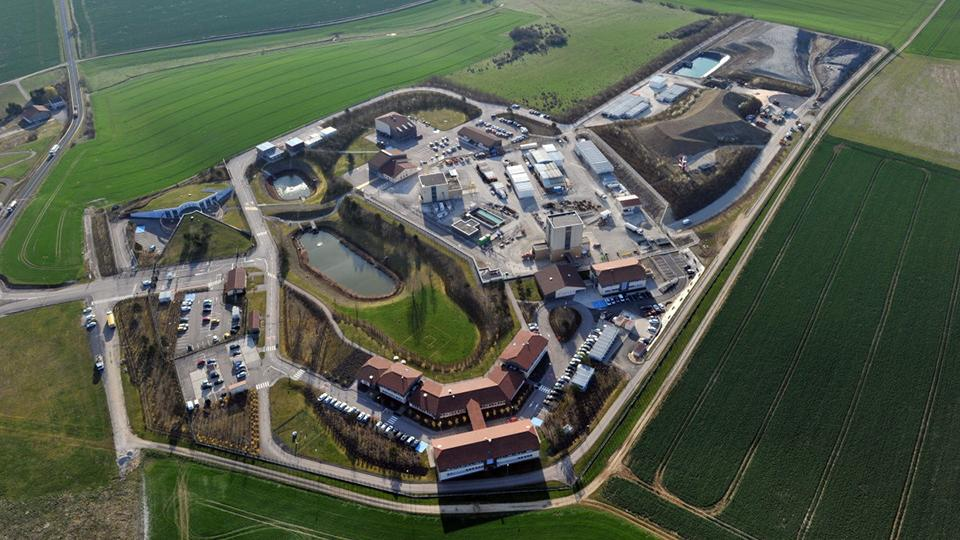
\includegraphics[width=\textwidth]{cigeo.jpg}
            \caption{Laboratoire souterrain de Bure}
        \end{figure}
    \end{columns}
\end{frame}

\begin{frame}{Architecture Matérielle Consolidée}
    \begin{columns}
        \column{0.5\textwidth}
        \begin{itemize}
            \item \textbf{Base :} Agilex Scout Mini (Odométrie roues).
            \item \textbf{Calcul :} Jetson Orin Nano (Inférence GPU).
            \item \textbf{Vision :} 
                \begin{itemize}
                    \item Caméra PTZ (Prises de vue haute résolution).
                    \item ZED2i (Données IMU pour l'EKF).
                    \item Caméra 360 (Acquisition globale).
                \end{itemize}
            \item \textbf{Positionnement :} LiDAR 2D YDLidar TG15.
        \end{itemize}
        \column{0.5\textwidth}
        \begin{figure}
            \centering
            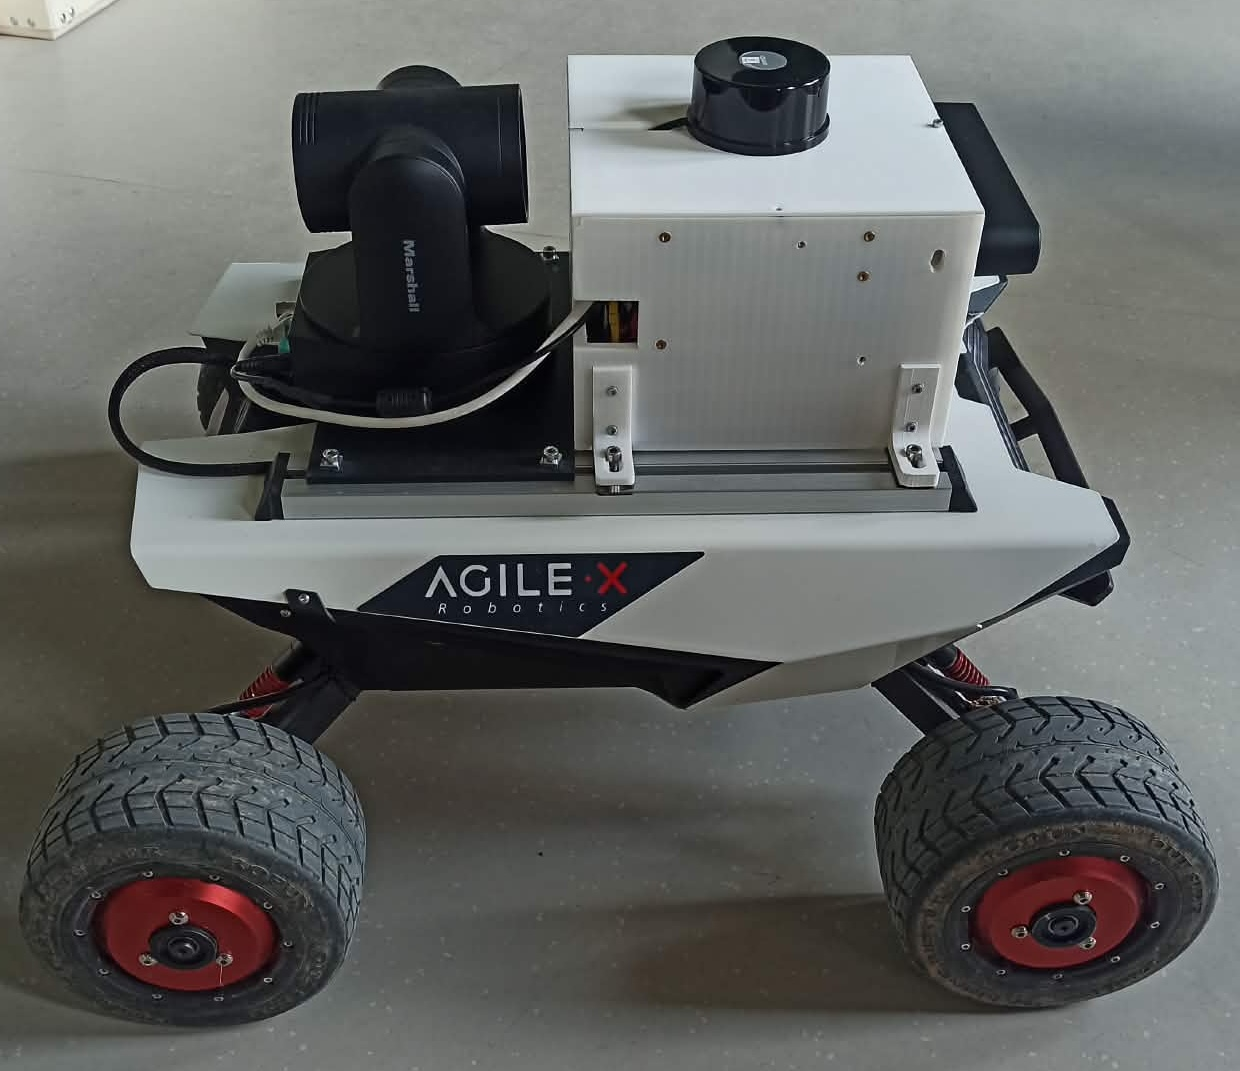
\includegraphics[width=0.8\textwidth]{montage_final.png}
            \caption{Robot dans sa configuration finale}
        \end{figure}
    \end{columns}
\end{frame}

% --- SECTION 2 : RÉSULTATS SEMESTRE 1 & PREMIÈRE DESCENTE ---
\section{Semestre 1 : Reconstruction et Première Descente}

\begin{frame}{Bilan de la Première Descente (Février 2026)}
    \begin{columns}
        \column{0.6\textwidth}
        \textbf{Succès :}
        \begin{itemize}
            \item Validation du socle \textbf{ROS2 Humble}.
            \item Hotspot Jetson opérationnel (SSH en tunnel).
            \item Première collecte de données 360°.
        \end{itemize}
        \vspace{0.2cm}
        \textbf{Défis identifiés :}
        \begin{itemize}
            \item[\textcolor{red}{\textbullet}] \textbf{Panne LiDAR :} Port micro-USB arraché.
            \item[\textcolor{red}{\textbullet}] \textbf{Drift :} Erreur de transformations TF (trajectoire non-planaire).
            \item[\textcolor{red}{\textbullet}] \textbf{Couverture :} Séquence PTZ 3 photos insuffisante.
        \end{itemize}
        \column{0.4\textwidth}
        \begin{figure}
            \centering
            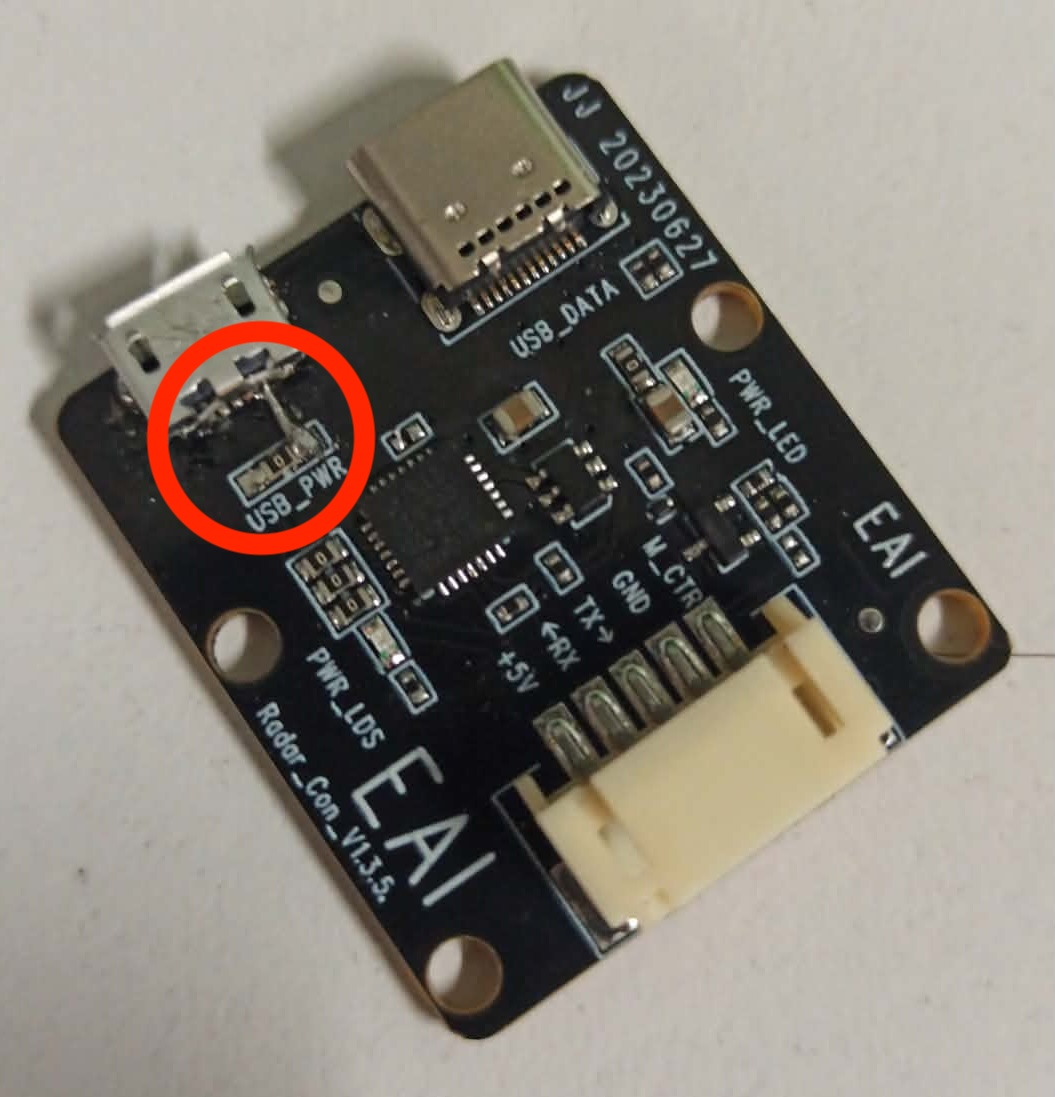
\includegraphics[width=0.6\textwidth]{chipset_lidar.jpg}
            \caption{Diagnostic du LiDAR cassé}
        \end{figure}
    \end{columns}
\end{frame}

% --- SECTION 3 : SEMESTRE 2 : RÉSOLUTIONS TECHNIQUES ---
\section{Semestre 2 : Optimisations et Navigation}

\begin{frame}{Résolution du problème LiDAR}
    \begin{columns}
        \column{0.6\textwidth}
        \begin{block}{Correction Matérielle}
            Abandon du micro-USB au profit d'un branchement de secours via \textbf{USB-C}.
        \end{block}
        \begin{block}{Correction Logicielle}
            Passage au driver \texttt{TG.yaml} (spécifique au TG15) et recalage du port série sur \texttt{/dev/ttyUSB0}.
        \end{block}
        \vspace{0.3cm}
        \textbf{Résultat :} Scan 360° fonctionnel, permettant enfin la cartographie et la localisation AMCL.
        
        \column{0.4\textwidth}
        \begin{figure}
            \centering
            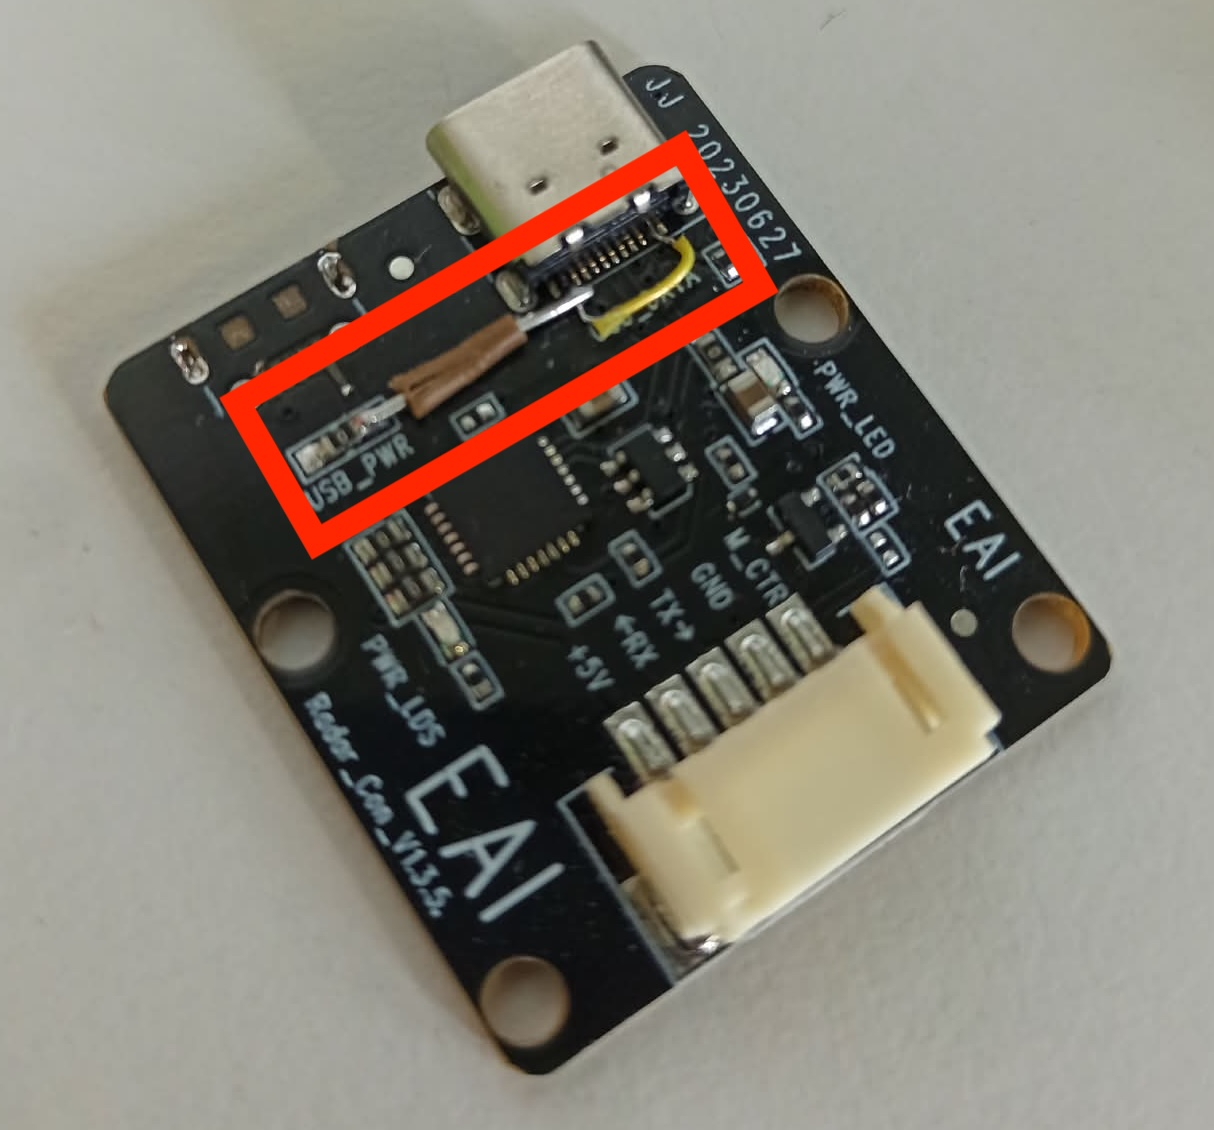
\includegraphics[width=0.8\textwidth]{chipset_lidar_repare.jpg}
            \caption{Réparation et nouveau câblage}
        \end{figure}
    \end{columns}
\end{frame}

\begin{frame}{Optimisation IA : TensorRT et Docker}
    Pour garantir une détection en temps réel sur la Jetson Orin Nano :
    \begin{itemize}
        \item \textbf{Conteneurisation :} Docker (\texttt{l4t-pytorch}) pour isoler les dépendances CUDA/ROS2.
        \item \textbf{TensorRT :} Conversion du modèle YOLOv11 (\texttt{.pt} $\rightarrow$ \texttt{.engine}).
    \end{itemize}
    \vspace{0.4cm}
    \begin{table}
        \centering
        \begin{tabular}{lcc}
            \toprule
            \textbf{Format du modèle} & \textbf{Vitesse d'inférence} & \textbf{Accélération} \\
            \midrule
            PyTorch Standard (.pt) & $\approx$ 5-8 FPS & 1x \\
            \textbf{TensorRT Engine (.engine)} & \textbf{$\approx$ 25-30 FPS} & \textbf{x4} \\
            \bottomrule
        \end{tabular}
        \caption{Gain de performance sur Jetson Orin Nano}
    \end{table}
\end{frame}

\begin{frame}{Évolution Mécanique et Qualité de Scan}
    \begin{columns}
        \column{0.5\textwidth}
        \textbf{Problématique :} 
        Les piliers de la tourelle masquaient le LiDAR, créant des angles morts pour la navigation.
        
        \vspace{0.3cm}
        \textbf{Solution :} 
        Création de platines \textbf{imprimées en 3D} pour surélever le LiDAR et déporter la PTZ à l'arrière.
        
        \column{0.5\textwidth}
        \begin{figure}
            \centering
            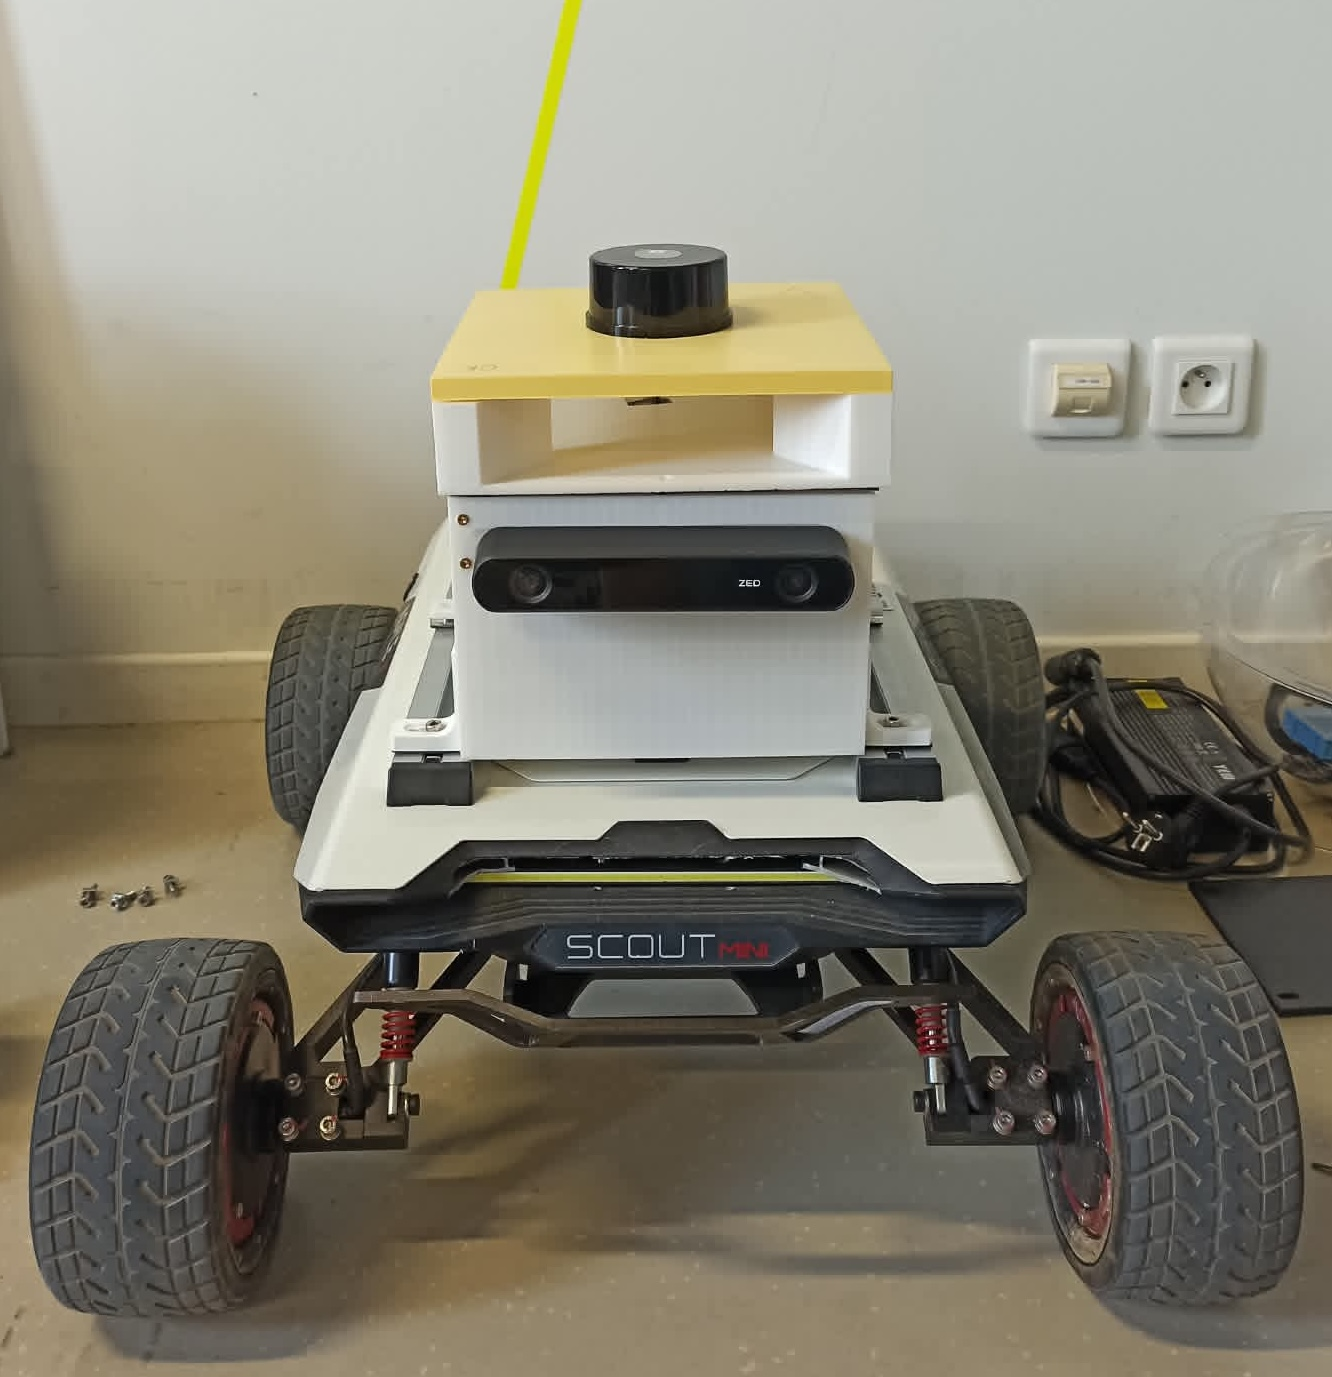
\includegraphics[width=0.8\textwidth]{premier_platine.jpg}
            \caption{Nouvelle platine LiDAR 3D}
        \end{figure}
    \end{columns}
\end{frame}

% --- SECTION 4 : NAVIGATION ET FUSION ---
\section{Navigation Autonome et Patrouille}

\begin{frame}{Navigation par Waypoints (Nav2)}
    \begin{columns}
        \column{0.6\textwidth}
        \begin{itemize}
            \item \textbf{Localisation :} AMCL recalé sur carte statique (.pgm).
            \item \textbf{Interface :} Utilisation de RViz (\texttt{2D Nav Goal}) pour définir les missions.
            \item \textbf{Autonomie :} Nœud \texttt{trajectoire\_mission.py} pour envoyer des poses successives.
        \end{itemize}
        \begin{block}{Stabilité TF}
            Fusion odométrie roues + IMU ZED2i via un filtre de Kalman étendu (EKF) pour une trajectoire planaire robuste.
        \end{block}
        \column{0.4\textwidth}
        \begin{figure}
            \centering
            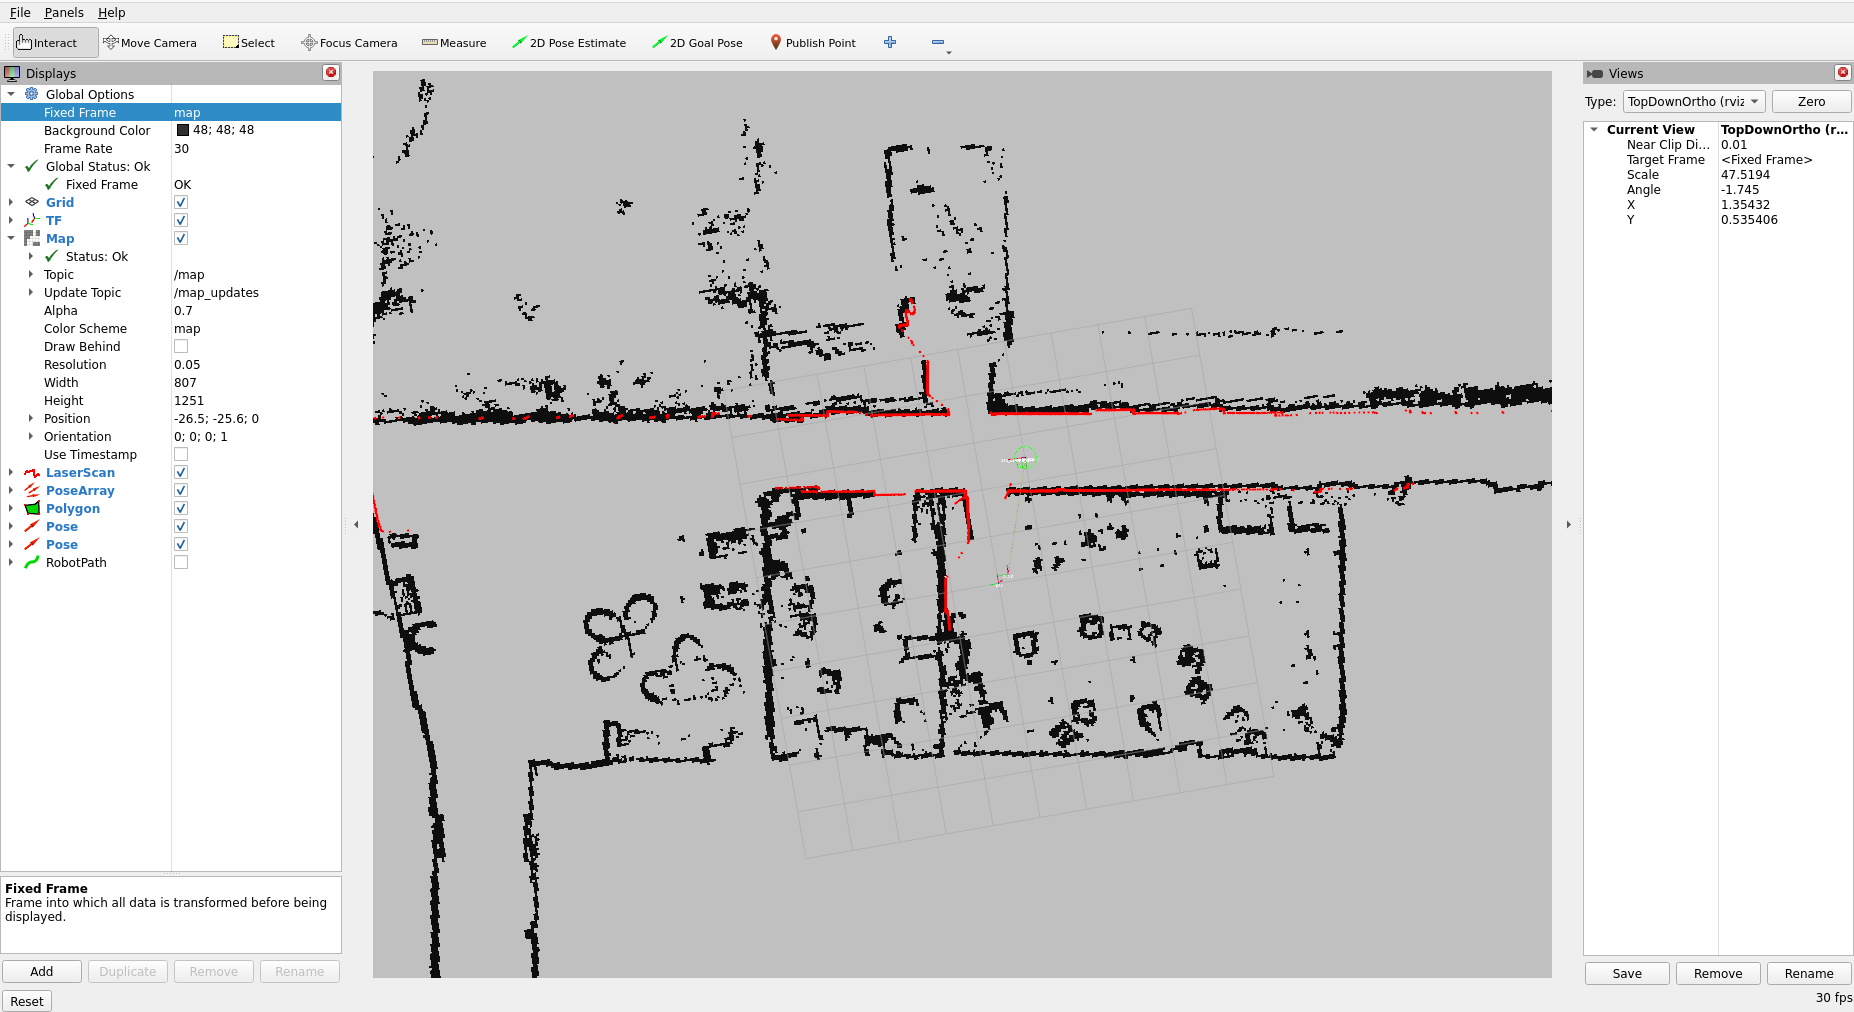
\includegraphics[width=\textwidth]{screen_rviz.png}
            \caption{Planification de mission sous RViz}
        \end{figure}
    \end{columns}
\end{frame}

\begin{frame}{Fusion : Navigation + Acquisition}
    \begin{block}{Package \texttt{patrouille\_autonome}}
        Orchestration synchrone du déplacement et de l'inspection.
    \end{block}
    
    \begin{columns}
        \column{0.5\textwidth}
        \textbf{Mode Photo-Navigation :}
        \begin{enumerate}
            \item Le robot atteint un waypoint.
            \item Arrêt complet et stabilisation.
            \item Séquence PTZ (5 photos pour l'arche).
            \item Reprise du mouvement.
        \end{enumerate}
        \column{0.5\textwidth}
        \textbf{Mode Vidéo-Navigation :}
        \begin{enumerate}
            \item Déplacement à vitesse très réduite.
            \item Enregistrement vidéo continu.
            \item Analyse différée ou en flux tendu via TensorRT.
        \end{enumerate}
    \end{columns}
\end{frame}

% --- SECTION 5 : BILAN ET CONCLUSION ---
\section{Bilan et Perspectives}

\begin{frame}{Résultats Finales et Cartographie}
    \begin{columns}
        \column{0.6\textwidth}
        \textbf{Résultats :}
        \begin{itemize}
            \item Système complet de détection optimisé (TensorRT).
            \item Navigation autonome par waypoints validée.
            \item Dataset 360° enrichi pour l'évolution future du modèle.
        \end{itemize}
        \vspace{0.3cm}
        \textbf{Limites persistantes :}
        \begin{itemize}
            \item Dérive (drift) résiduelle sur les très longues galeries.
            \item Cartographie SLAM encore perfectible en milieu symétrique.
        \end{itemize}
        \column{0.4\textwidth}
        \begin{figure}
            \centering
            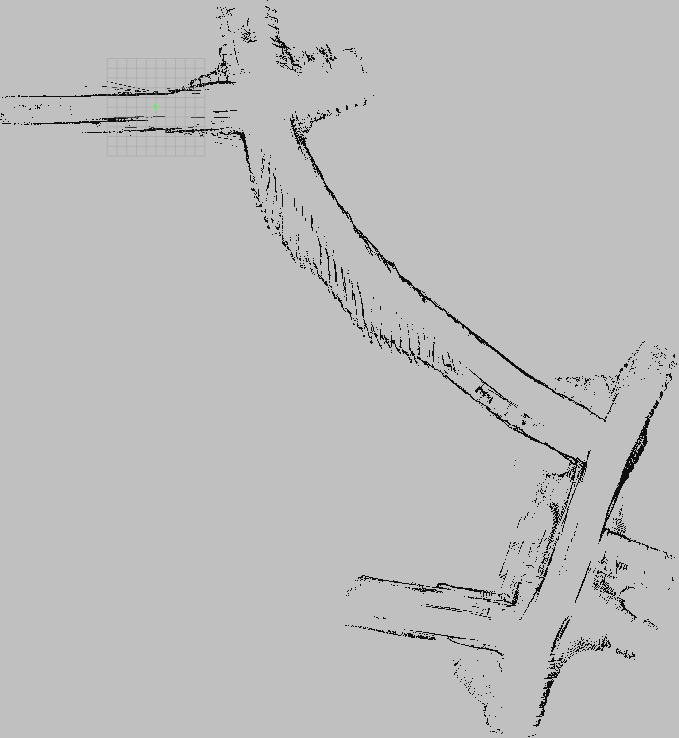
\includegraphics[width=0.9\textwidth]{test_andra.png}
            \caption{Scan LiDAR d'un tunnel}
        \end{figure}
    \end{columns}
\end{frame}

\begin{frame}{Conclusion et Ouvertures}
    \begin{block}{Bilan du projet}
        Transition réussie d'un robot télécommandé vers une plateforme autonome de patrouille capable d'inférence IA haute performance.
    \end{block}
    
    \vspace{0.5cm}
    \textbf{Perspectives :}
    \begin{itemize}
        \item \textbf{Vision 360 :} Finaliser l'entraînement YOLO sur les images panoramiques pour supprimer les arrêts PTZ.
        \item \textbf{SLAM 3D :} Passer sur une solution LiDAR 3D pour supprimer définitivement le drift vertical.
        \item \textbf{Interface IHM :} Développer une tablette de contrôle simplifiée pour les opérateurs ANDRA.
    \end{itemize}
    
    \vspace{0.8cm}
    \centering
    \Large \textbf{Merci de votre attention. Avez-vous des questions ?}
\end{frame}

\end{document}